\section{\textit{Reinforcement Learning}}

\textit{Reinforcement learning} (RL) merupakan sebuah kerangka pembelajaran sebuah kerangka pengembangan sebuah agen otonom yang dapat membuat suatu keputusan dalam ruang lingkup permasalahan yang terbatas. Secara umum, berikut merupakan formulasi sederhana dari kerangka \ac{RL}.

\begin{equation}
	\pi(s,a)^* = argmax(V(s,a))
\end{equation}

\(\pi\) merupakan notasi dari hasil fungsi kebijakan (\textit{policy}) yang merupakan keluaran dari \ac{RL}. Terdapat dua input untuk fungsi kebijakan tersebut, yaitu state (\(s\)) dan aksi (\(\alpha\)). Hasil yang diinginkan dari fungsi tersebut, adalah didapatkannya aksi yang terbaik dengan hasil evaluasi sebuah fungsi penilai (\(V\)). Berikut merupakan contoh dari penggunaan \ac{RL} pada Gambar \ref{fig:ilustrasi-RL} sebagai ilustrasi cara kerja fungsi kebijakan.

\begin{figure}[h]
	\centering
	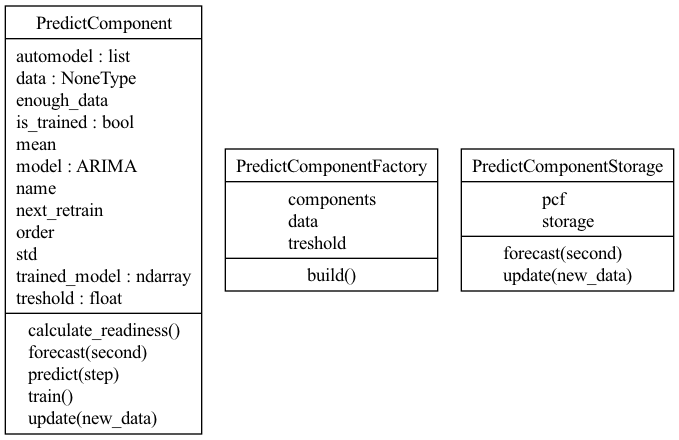
\includegraphics[width=0.8\textwidth]{chapter-4/predictor.png}
	\caption{Ilustrasi \ac{RL}}
	\label{fig:ilustrasi-RL}
\end{figure}

